\section*{Vitamina D}

La vitamina D es una hormona que proviene principalmente de la síntesis en la piel a través de la radiación solar (formando un 80-90\% de los requerimientos diarios de vitamina D), mientras que el resto es ingerido mediante la dieta en una pequeña cantidad de alimentos que la contienen, tales como los pescados grasos, las yemas de huevo, los lácteos fortificados y algunos tipos de hongos\cite{Holick_2010}.

La vitamina D se presenta de dos formas: D\textsubscript{2} (sintetizada a partir de ergosterol en plantas) y D\textsubscript{3} (sintetizada a partir de 7-dehidrocolesterol en mamíferos). Los humanos tenemos inserto el 7-dehidrocolesterol en la bicapa lipídica de la membrana plasmática de los queratinocitos de la epidermis y los fibroblastos de la dermis\cite{zuluga_2011}. Este compuesto tiene una estructura relativamente rígida de 4 anillos que, al exponerse a la radiación UVB, la energía contenida en la onda electromagnética provoca que el anillo B se abra, formando una estructura menos rígida que la anterior: la pre-vitamina D. Una vez formada, la pre-vitamina D rápidamente se transforma en la vitamina D\textsubscript{3} (o colecalciferol) que es termodinámicamente más estable. De esta manera, la vitamina D\textsubscript{3} es eyectada desde la membrana plasmática hacia el espacio extracelular. La proteína transportadora de vitamina D (DBP) en los capilares tiene una gran afinidad por la vitamina D3, de manera que la adentra en la circulación sanguínea\cite{Holick_1989}.

A través del torrente sanguíneo, la vitamina D\textsubscript{3} alcanza el hígado donde sufre una hidroxilación por la 25$\alpha$-hidroxilasa (enzima perteneciente al grupo de las citocromo P450), formando la 25(OH)D o calcidiol. Luego, se dirige a través del torrente sanguíneo hacia el riñón, órgano en el que se produce otra hidroxilación, esta vez en el carbono 1, obteniendo así la 1-25(OH)D, mejor conocida como vitamina D activa o calcitriol\cite{zuluga_2011}.

Esta forma activa tiene la capacidad de interactuar con el receptor de vitamina D (VDR), una proteína intracelular que se expresa en tejidos muy diversos en el cuerpo humano, tales como intestino delgado, colon, hueso, glándula paratiroidea,  piel, pulmones, entre otros.

En consecuencia, la vitamina D tiene múltiples efectos que podemos dividir en clásicos y no clásicos\cite{bikle_2014}. Los clásicos y más conocidos se dan en el metabolismo fosfo-cálcico mediante el aumento de la absorción de calcio a nivel intestinal, el incremento del recambio óseo y de la reabsorción renal de calcio y fosfato\cite{zuluga_2011}. Por otro lado, se le han atribuido acciones no clásicas, entre las que se encuentra la inmunomodulación, la regulación de la actividad de las células neoplásicas y el control de la presión arterial\cite{atlas_radiacion_colombia_2005}. Además, el déficit de esta hormona está asociado a distintas patologías como la sarcopenia\cite{atlas_radiacion_colombia_2005}, la preeclampsia\cite{belizan_1991} y artritis reumatoidea\cite{Ishikawa_2016}; y se ha correlacionado incluso a un mayor riesgo en la enfermedad causada por el COVID-19\cite{Mercola2020}.

La síntesis de vitamina D en la piel humana producida por la radiación solar es la principal fuente de vitamina D en los seres humanos, ya que su ingesta aporta solo el 10\% del suministro necesario\cite{adam_2002}. Por lo tanto, cualquier factor que altere la llegada de la radiación solar UV a la piel se ve reflejado en la producción de vitamina D\textsubscript{3}\cite{Holick_2004}.

\section*{Índice UV}

El sol emite radiación electromagnética, clasificada de acuerdo a su longitud de onda ($\lambda$). La intensidad de la radiación solar que llega a la superficie terrestre depende de la ubicación geográfica, la hora del día, los días del año y de la composición atmosférica. El rango más energético corresponde al ultravioleta (UV), el cual se divide en UVB (280-320 nm) y UVA (320-400 nm). La radiación solar UV es atenuada principalmente por los diferentes gases y partículas que componen la atmósfera\cite{Hrabk_2018}. Entre los más importantes se encuentran el ozono (O3) y la profundidad óptica de aerosoles (AOD por su acrónimo en inglés)\cite{Kazadzis_2009}, mientras que en menor medida influyen el dióxido de azufre (SO2) y dióxido de nitrógeno (NO2)\cite{Bais_1993}.

Los efectos biológicos de la radiación UV son descritos a través de un espectro de acción S($\lambda$). En particular, el espectro de acción eritémico representa la sensibilidad de la piel humana para producir eritema. Para determinar la capacidad de una fuente UV (280-400 nm) para generar eritema se emplea la siguiente relación:

\begin{equation*}
    E_{er} = \int\limits_{280nm}^{400nm} E(\lambda,t)S_{er} (\lambda) d\lambda \label{eq:eer}
\end{equation*}

Donde E\textsubscript{er} es la irradiancia eritémica, $E(\lambda,t)$ es el espectro solar y $S(\lambda)$ es el espectro de acción eritémica. A partir de multiplicar Eer por 40m\textsuperscript{2}/W se obtiene el Índice UV (IUV), una cantidad adimensional e internacionalmente reconocida para medir el riesgo de producir eritema en una escala de 0 a 20 (o más). Por otro lado, la Dosis Mínima Eritémica (DEM) se define como:

\begin{equation*}
    DEM = \frac{1}{4} \int\limits_{t_1}^{t_2}IUV dt
\end{equation*}

donde t$_2$-t$_1$ es el tiempo de exposición solar (TES) para alcanzar una DEM. La DEM adquiere diferentes valores de acuerdo al fototipo de piel. En la clasificación de Fitzpatrick los fototipos se definen del más claro (I) al más oscuro (VI), siendo este último el de mayor tolerancia a la radiación UV. La DEM es la dosis efectiva (en unidades de J/m$^2$) de acuerdo a cada fototipo, para producir eritema sin exposición previa\cite{CIE_2014}. La DEM estándar corresponde a un valor de 250 J/m$^2$, para una persona de fototipo de piel II\cite{CIE_2014}. Por otro lado, de manera análoga se estableció que la Dosis mínima UV ponderada con la tasa de producción de pre-vitamina D por día (DDM), es la requerida para mantener una cantidad adecuada de vitamina D2. La DDM para una persona con fototipo II, en una exposición solar del 25\% del cuerpo (brazos, manos y cara), tiene un valor aproximado de $\frac{1}{4}$ DEM al mediodía solar\cite{Dowdy_2010}. En el presente trabajo se utiliza como referencia en el cálculo, el valor de 1 DDM= $\frac{1}{4}$ DEM = 63 J/m$^2$.

\section*{Quema de pastizales en las Islas del Delta}

El año 2020 marcó a los habitantes de la ciudad de Rosario y zonas aledañas por las cifras récord de incendios ocurridos sobre los humedales cercanos a este territorio. Las Islas del Delta del Paraná comprenden los macrosistemas de humedales de origen fluvial que se extienden desde la ciudad de Diamante (Provincia de Entre Ríos) hasta la Ciudad Autónoma de Buenos Aires, recorriendo aproximadamente 300 km de largo y confluyendo junto al Río Uruguay en el estuario del Río de la Plata. Los humedales ocupan una superficie de aproximadamente dos millones de hectáreas, calificadas como zonas bajas e inundables\cite{acuario_del_rio_parana}. Esta región es explotada para diversas actividades económicas, principalmente aquellas relacionadas a la ganadería y la agricultura\cite{Galperin_2013}. El Servicio Nacional del Manejo del Fuego reportó que el 95\% de los incendios que ocurren en Argentina son producto de intervenciones humanas\cite{SNMF_2020}.

La quema de pastizales como método de barrido para el rebrote de especies forrajeras, se ha implementado desde hace más de dos siglos en regiones tropicales y subtropicales del continente americano\cite{quemas_2008,SNMF_2020,molinas_2020,atlas_radiacion_colombia_2005,henry_2010}. A pesar de que la problemática no es reciente, esta se acentuó a finales del siglo XX cuando Argentina aplicó cambios del uso de suelo, desplazando el pastoreo hacia los humedales del río Paraná\cite{vazquez_2017}. A partir de la introducción de ganado a las islas, el uso del fuego como intermediario en la remoción de vegetación se aplica anualmente durante los meses de invierno  (época en la cual típicamente tanto la humedad ambiente como la temperatura son bajas y las precipitaciones son menores que en el resto del año)\cite{global_solar_uv_index_2002}.

En el año 2019, la combinación de incendios clandestinos y la extrema sequía, devastaron miles de hectáreas del Amazonas\cite{Estupin_1996,Holick_1989}. Durante la temporada invernal del año siguiente la sequía se prolongó y el río Paraná tuvo su nivel más bajo en los últimos 50 años. Particularmente entre Junio y Agosto 2020 se registraron solo 12 días de lluvia, menos de la mitad de la precipitación medida una década atrás. Todos estos factores contribuyeron a que en el 2020 se registraran cifras récord de incendios en las islas del Delta del río Paraná\cite{Holick_2004}. En total, se estima que se consumieron alrededor de 300.000 ha. de la superficie de las Islas del Delta\cite{pagina_12}, es decir, 4 veces más que lo calculado en el antecedente del 2008\cite{quemas_2008}.

A pesar de este largo historial, al presente la única referencia que cuantifica el impacto en la calidad del aire producido por la biomasa quemada y los aerosoles emitidos hacia las ciudades del cordón Rosario-Buenos Aires data del año 2008\cite{Chameides1999}.

Los gases y el material particulado (o aerosoles) emitidos por las quemas de biomasa deterioran tanto la calidad del aire como la salud de las personas. El material particulado de tamaño menor a 2.5 micrones (PM\textsubscript{2.5}) al ingresar por las vías respiratorias tiene diferentes efectos perjudiciales: reduce la capacidad de transportar y liberar oxígeno a los tejidos a través de la sangre, genera injuria pulmonar e irritación en los tejidos oculares. El PM\textsubscript{2.5} también puede generar cambios en la información genética, lo que puede favorecer el desarrollo de cáncer en diversos tejidos\cite{molinas_2020}. Durante eventos de incendios forestales, las enfermedades respiratorias como el asma o la influenza muestran un incremento de los casos, exacerbadas por la alta concentración de aerosoles. Asimismo, existen proyecciones que prevén aumentos similares para los casos de COVID-19\cite{CIE_2014}.

La evidencia del efecto de la contaminación del aire sobre la síntesis de la vitamina D es todavía muy limitada. No obstante, se ha reportado que la deficiencia de la vitamina D tiene mayor incidencia en áreas contaminadas que en aquellas no contaminadas [Elham Feizabad et al. 2017]. La exposición prolongada a una mala calidad del aire también ha sido asociada a bajos niveles de esta vitamina (Chenlu Yang et al. 2021). A pesar de que la quema de biomasa frente a la ciudad de Rosario ocurre cada año y desde hace varias décadas, al presente no existen estudios sobre su impacto en la vitamina D adquirida vía solar. En este trabajo se analiza la influencia de los aerosoles producidos por los incendios en el Delta del río Paraná del año 2020 sobre las dosis diarias de vitamina D generadas vía solar.

\section*{Objetivos}

\subsection*{General}

Realizar una estimación del efecto de la contaminación atmosférica, principalmente los aerosoles propagados por el humo, producidos por los incendios en el Delta del Paraná en el año 2020 y que afectan las dosis de vitamina D adquiridas vía solar.

\subsection*{Especificos}

\begin{itemize}
    \item Identificar las fechas de cielo despejado en el periodo Junio-Agosto 2020. Posteriormente seleccionar los días críticos con gran número de focos de incendios y humo frente a la ciudad de Rosario, utilizando imágenes satelitales FIRMS-NASA.

    \item Seleccionar los valores del Índice UV medidos al mediodía por la estación meteorológica Davis del IFIR-CONICET-UNR, para los días críticos encontrados.

    \item Calcular el Índice UV al mediodía para los días críticos, en situación libre de contaminación o humo (con un AOD típico) empleando el modelo TUV.

    \item Determinar los Tiempos de Exposición al Sol (TES) que tardan en acumular las DDM (en J/m$^2$) para síntesis de vitamina D con y sin presencia de humo.

    \item Analizar las diferencias en los TES para alcanzar los niveles de 25(OH)D de acuerdo a lo reportado en literatura (Rodríguez Sangrador et al. 2011).
\end{itemize}

\section*{Material y métodos}

Se consideraron los días de cielo despejado (sin nubosidad) para evaluar la disminución de los valores de Índice UV debido a la presencia de aerosoles y su impacto en los TES para alcanzar las dosis de vitamina D. Para realizar esta estimación se utilizaron las siguientes herramientas:

\begin{enumerate}
    \item Estación meteorológica. Las mediciones de Índice UV diarias al mediodía solar, son registradas por la estación meteorológica Davis ubicada en el Instituto de Física Rosario (CONICET-UNR), en la ciudad de Rosario.

    \item Modelo computacional. El modelo Tropospheric Ultraviolet Radiation (TUV) es un programa que calcula los valores de Índice UV de acuerdo a las condiciones climáticas y las coordenadas geográficas del sitio de interés (latitud, longitud y altura sobre el nivel del mar). En particular se utilizaron datos de ozono del satélite OMI-AURA-NASA (\url{disc.gsfc.nasa.gov}).

    \item Imágenes satelitales. En la región del Delta del río Paraná los incendios son captados satelitalmente a una dada hora del día y pueden ser visualizados en la plataforma FIRMS-NASA (\url{https://firms.modaps.eosdis.nasa.gov/}). Estas imágenes permiten identificar los días con mayor cantidad de humo.
\end{enumerate}

Para cuantificar los efectos de la contaminación del aire sobre las DDM durante los incendios se utilizaron mediciones del Índice UV de la ciudad de Rosario. Las imágenes satelitales del periodo Junio-Agosto 2020, en las cuales se localizaron un alto número de focos de incendios en el Delta del río Paraná, fueron empleadas para seleccionar los días críticos (que fueron 31 en total, sobre 92 días analizados) y las mediciones del Índice UV correspondientes afectadas por la presencia de aerosoles. Para las mismas fechas se calculó con el modelo TUV, el Índice UV en situación de cielo despejado y libre de humo. A partir de los valores de Índice UV se derivaron los TES con y sin presencia de humo para las DDM. Los TES corresponden al tiempo en acumular $\frac{1}{4}$ DEM (o un DDM) comenzando la exposición en el máximo de intensidad solar (cerca del mediodía).

\section*{Resultados}

La selección de las mediciones de IUV con mayor presencia de contaminación fue realizada por medio de las imágenes satelitales diarias. Solo fueron considerados los días críticos donde se demostró presencia de humo en las ciudades proveniente de los focos de incendio (Figura \ref{fig:satelite}).

\begin{figure}[H]
    \centering
    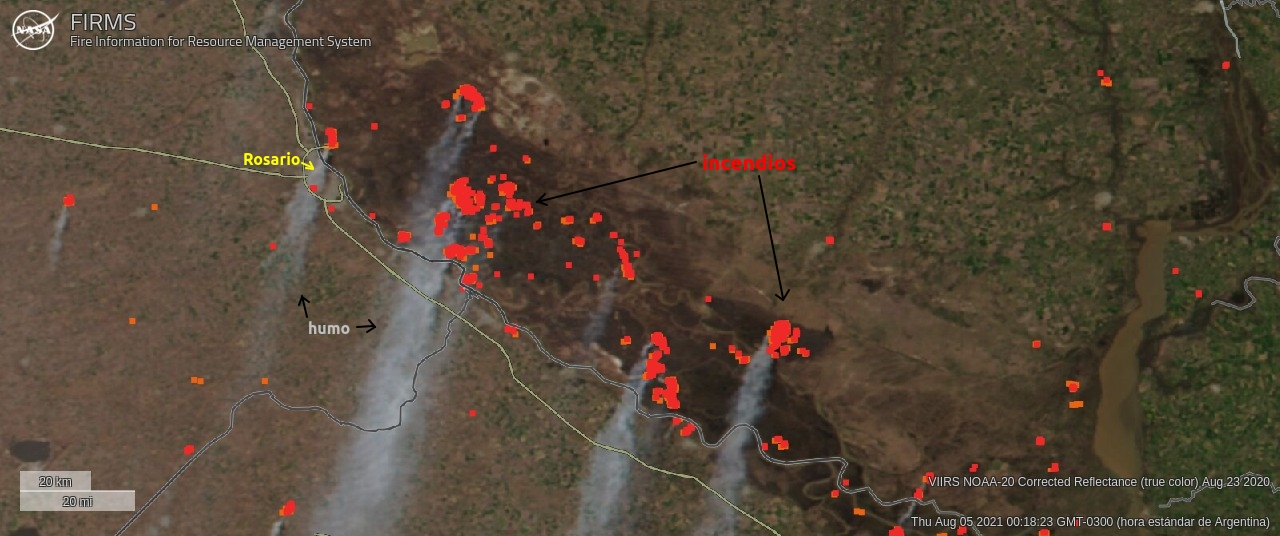
\includegraphics[width=12cm]{Graphics/image13.jpg}
    \caption{Imagen satelital FIRMS-NASA-NOAA tomada el 23 de agosto de 2020 en la región del Delta del río Paraná. Rosario recibiendo el humo arrastrado por el viento del Noreste (zonas grises) producido por los incendios (puntos rojos) sobre los humedales.}
    \label{fig:satelite}
\end{figure}

\begin{figure}[H]
    \centering
    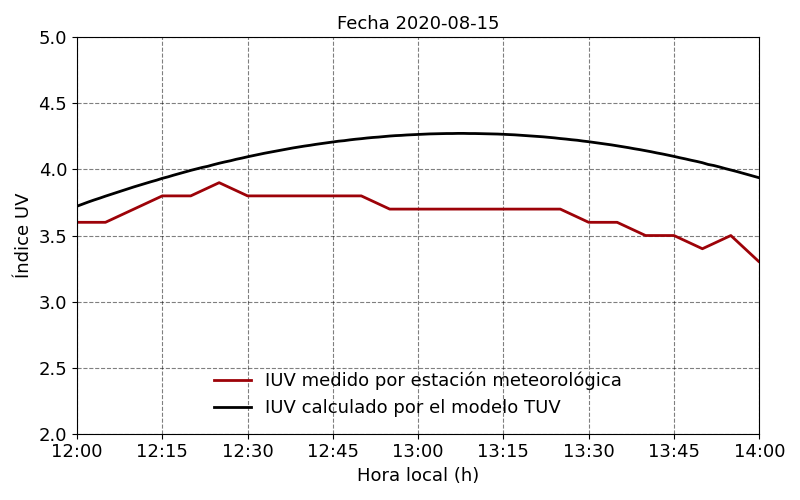
\includegraphics[width=12cm]{Graphics/image10.png}
    \caption{Índice UV medido por la estación meteorológica Davis y calculado por el modelo TUV para el 15 de agosto de 2020.}
    \label{fig:uvi_tuv}
\end{figure}

El Índice UV se estimó diariamente en el periodo Junio-Agosto 2020 para condiciones de cielo despejado y libre de humo. Estos valores fueron utilizados para obtener las DDM y los TES correspondientes. Para las fechas seleccionadas (31 días críticos con presencia de humo), este procedimiento se repitió calculando los TES por medio de las mediciones de Índice UV (ver ejemplo en Figura \ref{fig:uvi_tuv}). En la Figura \ref{fig:dr} se representan ambos conjuntos de los intervalos de tiempo hasta acumular 1 DDM, los cuales comienzan alrededor del mediodía solar (12:50 - 13:10h). Los TES para las fechas seleccionadas entre la última semana de Junio y primeros días de Julio son relativamente similares. Esto probablemente se debe a que en ese periodo se registraron dos días de lluvia, que barrieron la contaminación del aire provocada por los incendios. Además, en ese lapso la cantidad de incendios detectada fue la más baja de todo el periodo analizado y sólo 3 días los vientos tuvieron dirección (Norte, Noreste, Este) hacia la ciudad de Rosario. La segunda mitad del mes de Julio registró mayor cantidad de humo asentado en la región provocando un impacto significativo en la disminución del Índice UV y por lo tanto en las dosis asociadas. Se puede observar un aumento de los valores de los TES en ese periodo, ocasionado por una mayor presencia de humo/aerosoles, mientras que los TES calculados para situación normal fueron insuficientes para adquirir la DDM.

\begin{figure}[H]
    \centering
    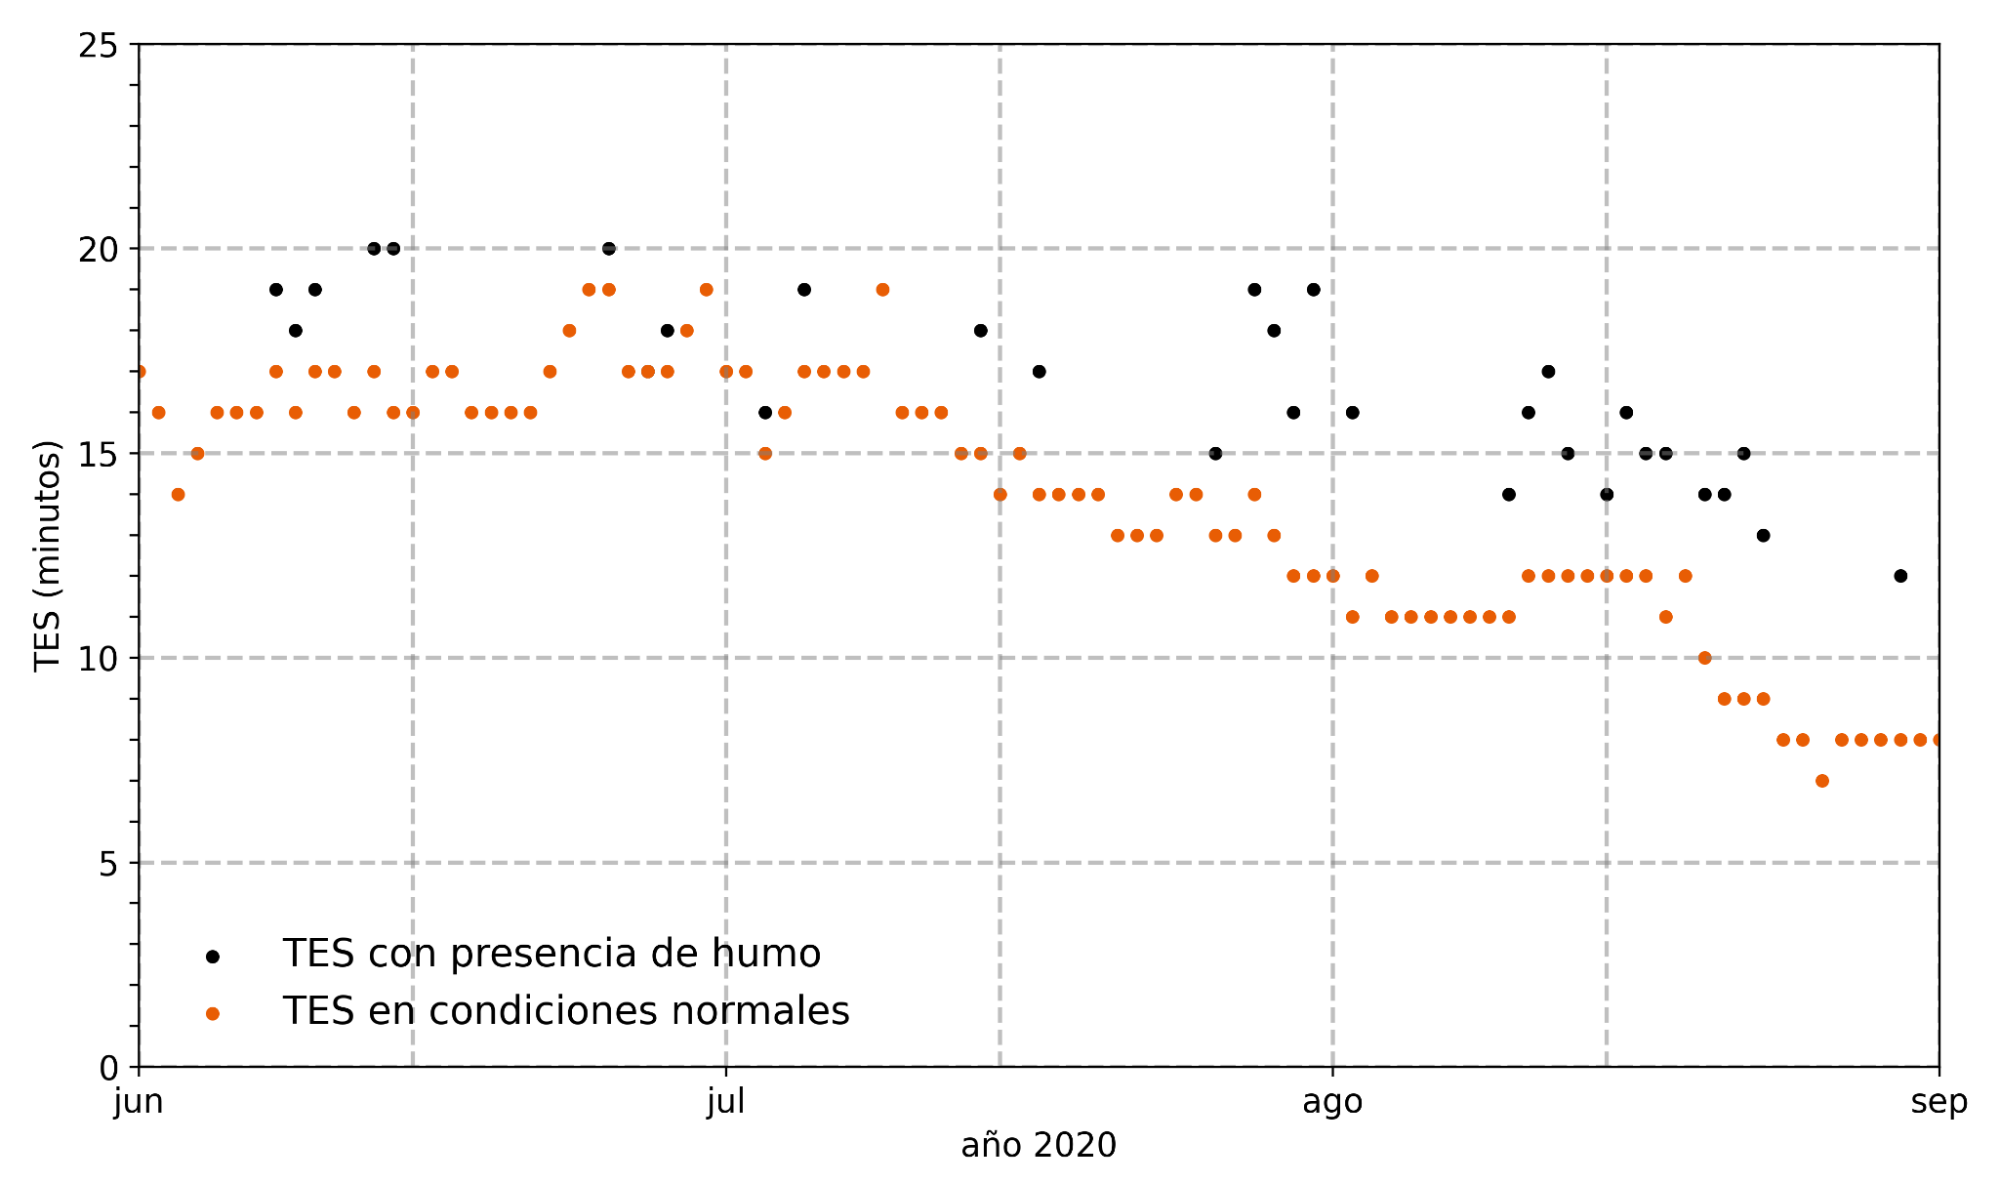
\includegraphics[width=8.2cm]{Graphics/image12.png}
    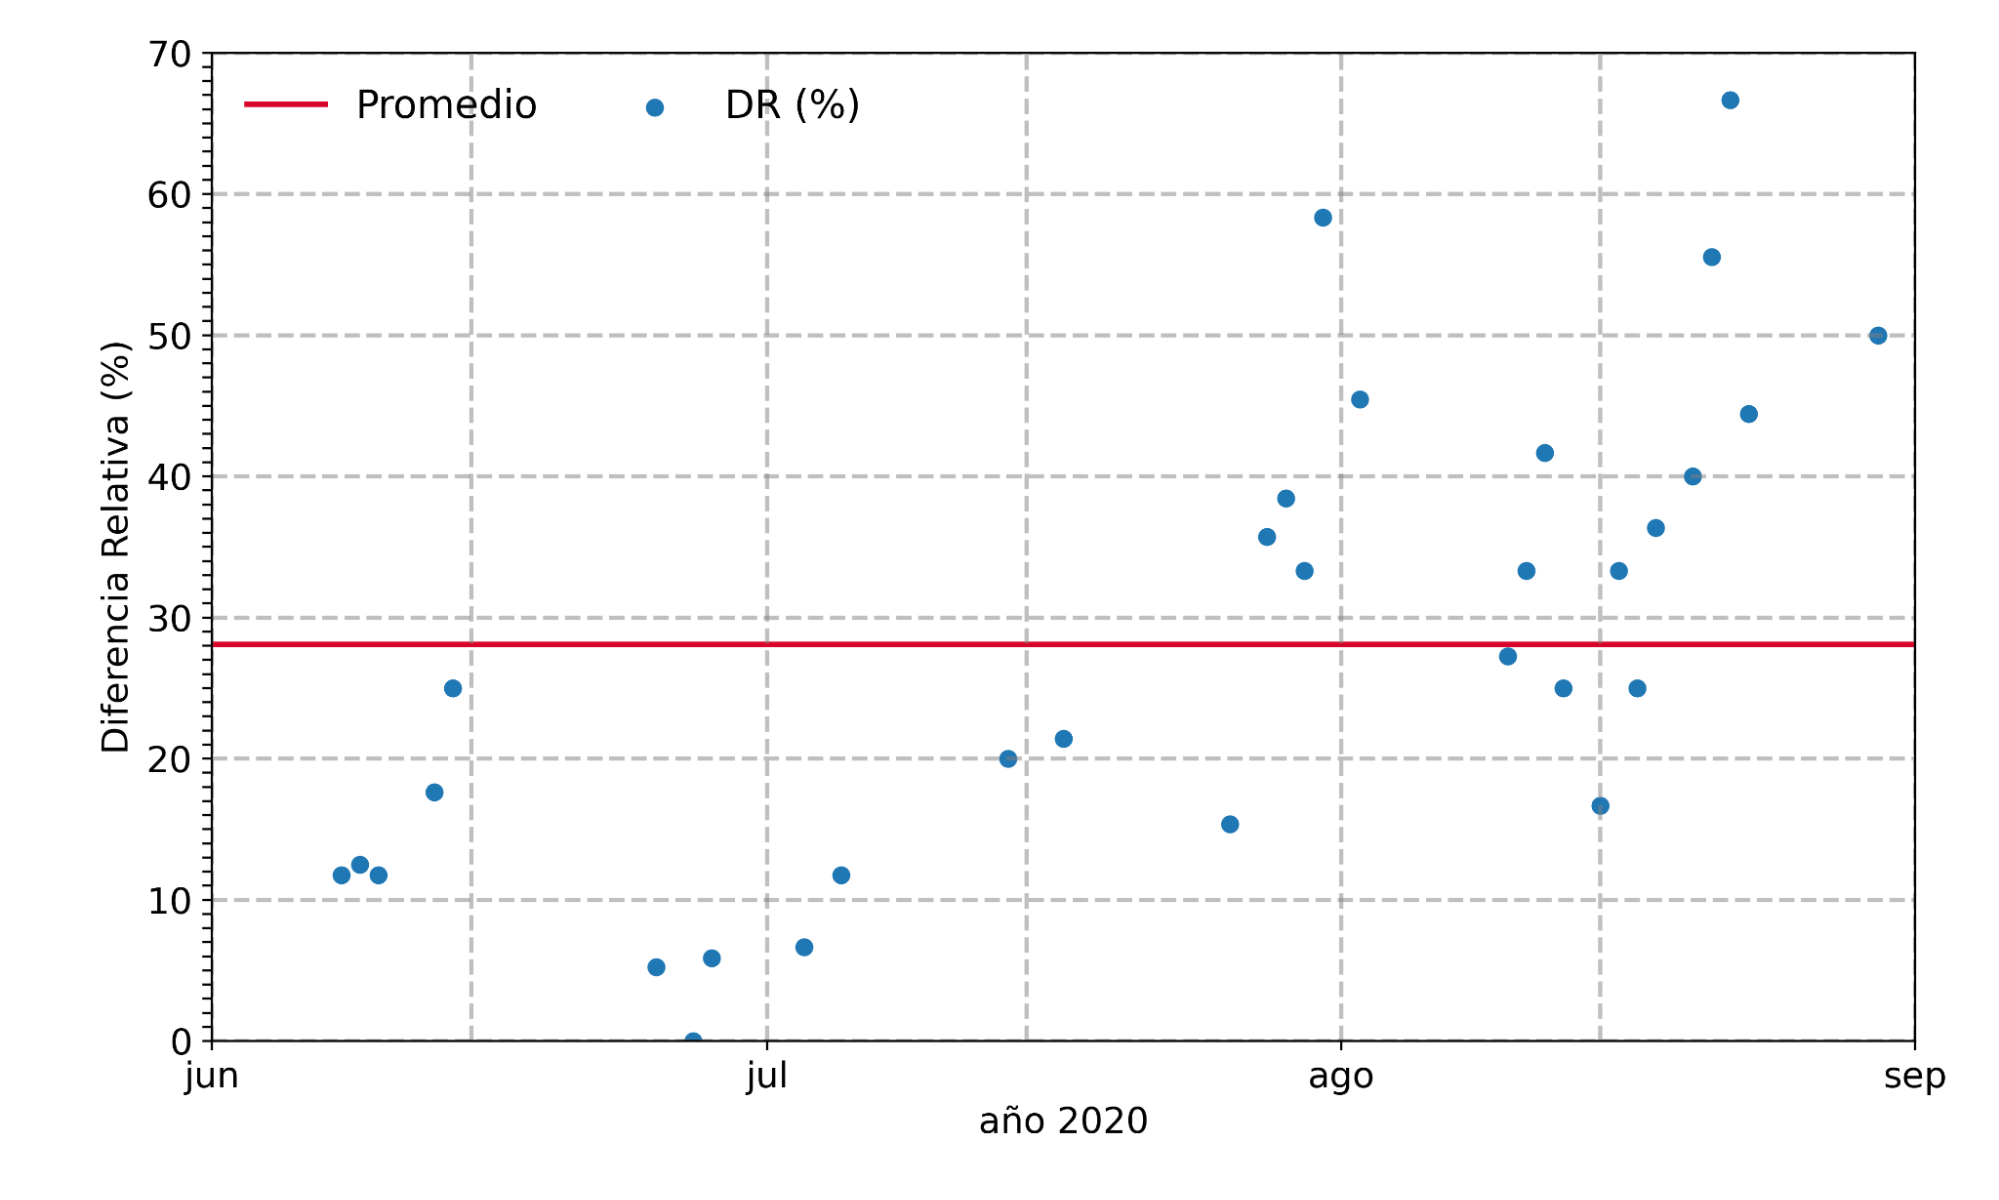
\includegraphics[width=8.2cm]{Graphics/image11.png}
    \caption{Izq. Tiempos de Exposición Solar (TES) en Rosario, para acumular una DDM: con presencia de humo (puntos negros) y en condiciones normales (puntos naranjas), durante el periodo Jun-Ago 2020. Diferencia relativa porcentual (DR\%) entre los TES coincidentes para las mismas fechas y su promedio (línea roja; 28.1\%).}
    \label{fig:dr}
\end{figure}

En la Figura \ref{fig:dr} se muestran las diferencias relativas porcentuales (DR\%) entre los TES calculados a partir de las mediciones afectadas por el humo y las estimaciones para condiciones normales del aire.

\begin{equation*}
    DR\% = \left(\frac{TES_{humo}-TES_{normal}}{TES_{normal}}\right)*100
\end{equation*}

Las DR\% tienen una tendencia creciente después de la segunda quincena de Julio hasta finales de Agosto. Este hecho coincidió con el registro de cifras récord en el número de focos de incendio y la reducción significativa de precipitación (50\% respecto a los últimos 5 años).

La correlación entre ambas condiciones atmosféricas en la ciudad de Rosario es mostrada en la Figura \ref{fig:regresion_lineal}. La pendiente de la recta que pasa por el origen fue de 1.22, indicando un incremento en los TES con presencia de humo.

\begin{figure}[H]
    \centering
    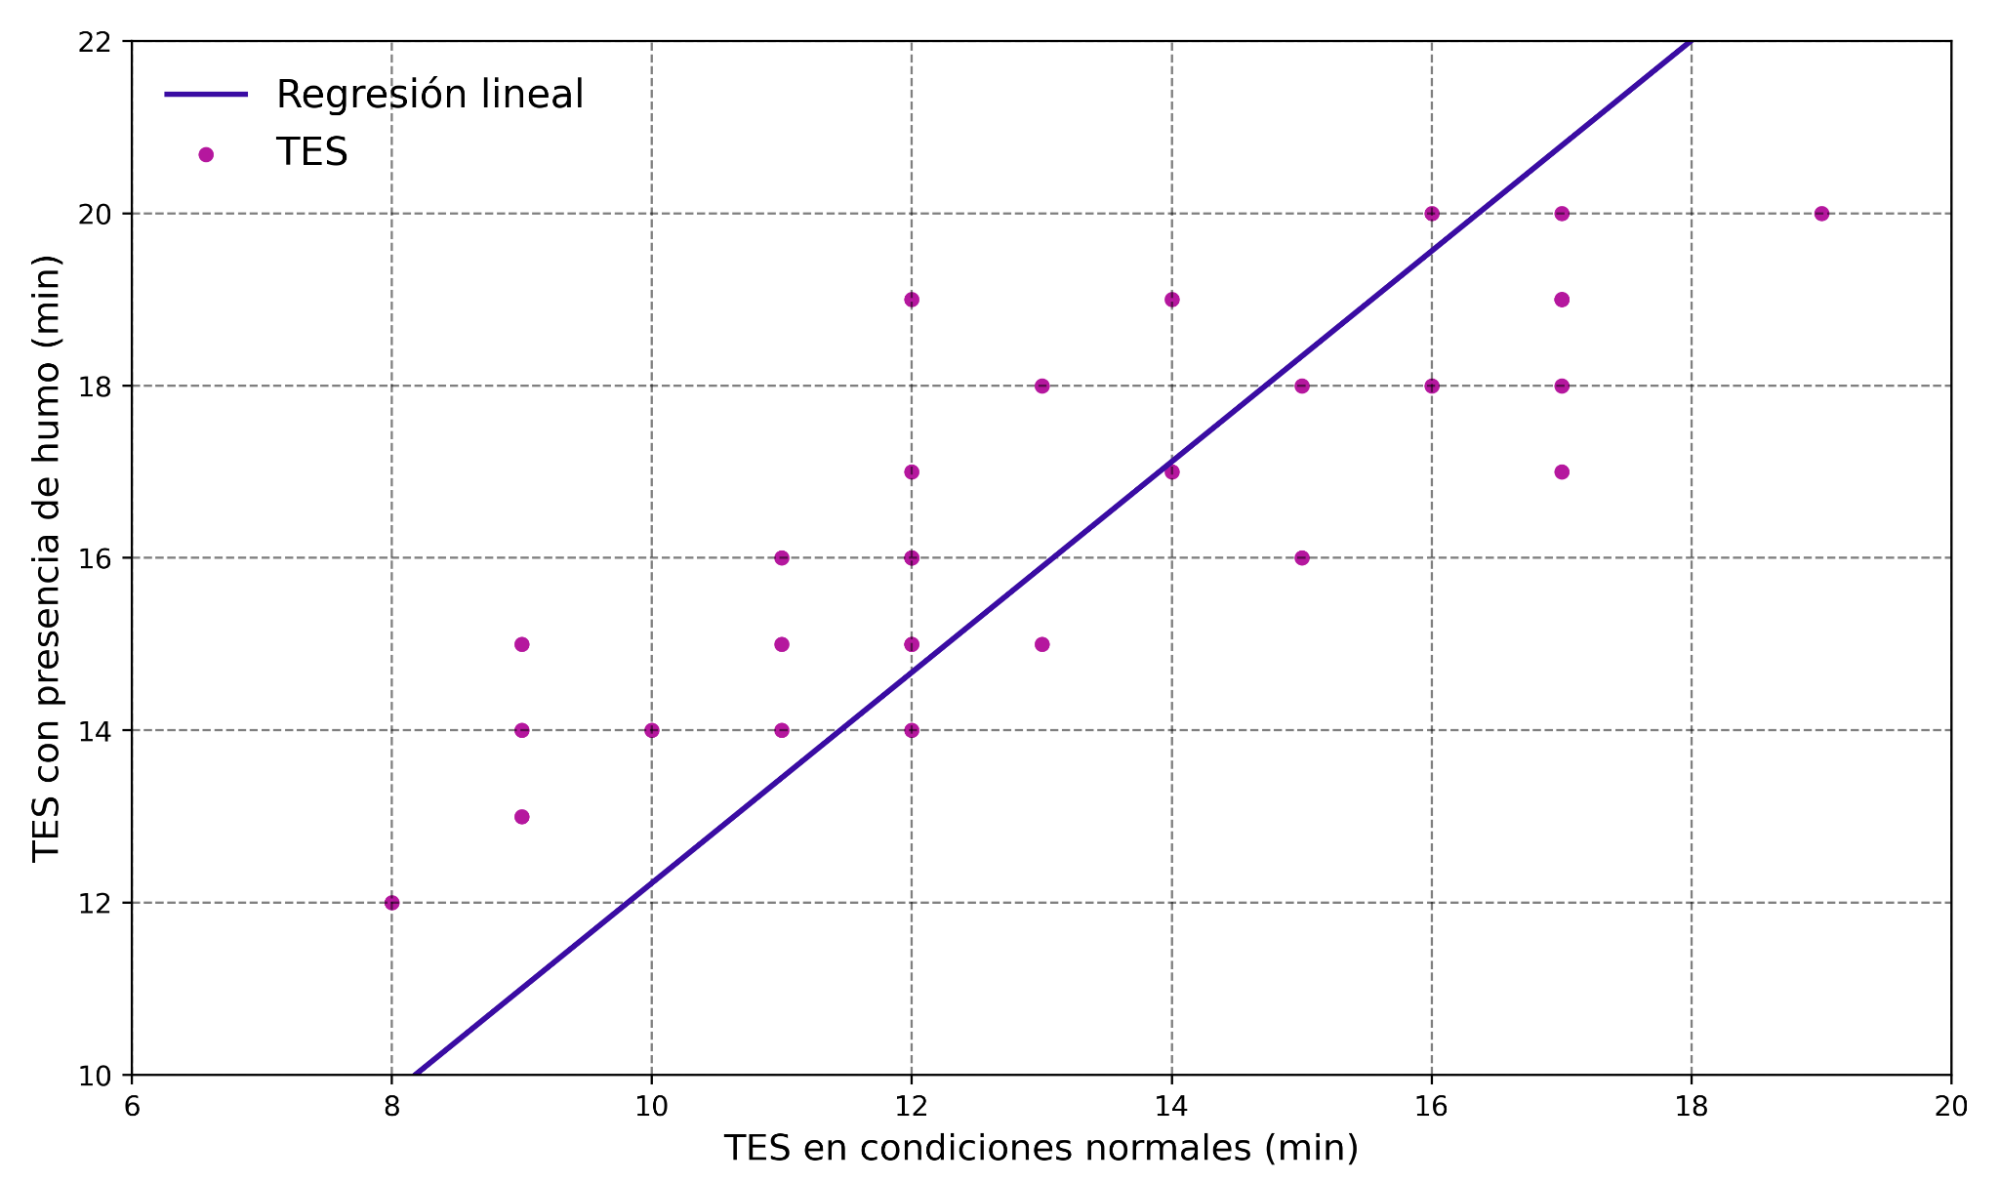
\includegraphics[width=12cm]{Graphics/image9.png}
    \caption{TES calculados  para los días seleccionados en el periodo Junio-Agosto 2020 en dos situaciones: Con presencia de humo y en condiciones normales (puntos magenta). Regresión lineal (línea morada) entre ambos casos, y= 1.22x.}
    \label{fig:regresion_lineal}
\end{figure}

A partir de las fechas seleccionadas como días críticos, se determinó el promedio de los TES en el periodo Junio-Agosto 2020. Los resultados se muestran en la Tabla 1 para los TES necesarios en acumular las DDM de 63 J/m$^2$ al mediodía solar en condiciones normales. La sumatoria de estas dosis diarias a lo largo de un total de 31 días (1953 J/m$^2$) derivaron los TES en ambas situaciones y una diferencia de 25\%. Rodríguez Sangrador et al. 2011 relacionó los hábitos de exposición solar con la concentración de 25(OH)D, reportando que durante 7 días de verano, adolescentes con dosímetros personales acumularon una dosis eritémica de 1519 J/m$^2$ y un promedio de 24.62 ng/ml. Para propósitos comparativos se utilizó esta relación de DEM acumulada, la cual fue alcanzada a los 25 días (ver Tabla \ref{table:TES}).

\begin{table}[H]
    \centering
    \begin{tabular}{|c|c|c|c|}
        \hline
        \multicolumn{1}{|l|}{\multirow{2}{*}{\textbf{Situación del aire ambiente}}} & \multicolumn{3}{c|}{\textbf{\begin{tabular}[c]{@{}c@{}}Tiempos de Exposición Solar para días críticos\\  durante el periodo Junio-Agosto 2020\end{tabular}}}                                                                                                                                                        \\ \cline{2-4}
        \multicolumn{1}{|l|}{}                                                      & \begin{tabular}[c]{@{}c@{}}Dosis 63 J/m$^2$\\ promedio\end{tabular}                                                                                            & \begin{tabular}[c]{@{}c@{}}Dosis acumulada\\ 1953 J/m$^2$\\ 31 días\end{tabular}                                 & \begin{tabular}[c]{@{}c@{}}Dosis acumulada*\\ 1519 J/m$^2$\\ 25 días\end{tabular} \\ \hline
        Normal                                                                      & 13 ± 3 min                                                                                                            & 6 h 52 min                                                 & 5 h 9 min                  \\ \hline
        con humo                                                                    & 17 ± 2 min                                                                                                            & 8 h 34 min                                                 & 6 h 38 min                 \\ \hline
        DR(\%)                                                                      & 30                                                                                                                 \% & 25                                                      \% & 29 \%                      \\ \hline
    \end{tabular}
    \caption{Comparación de los TES y sus DR\% para situación del aire ambiente: normal y con presencia de humo para días seleccionados en el periodo Junio-Agosto 2020.}
    \label{table:TES}
\end{table}

La DR\% entre los TES calculados para ambas situaciones de cielo se encuentran entre el 25-30\%. Es esperable que los TES tengan valores relativamente cortos debido a que son obtenidos a partir del máximo. Sin embargo, los niveles de Índice UV al mediodía en invierno en la ciudad de Rosario son muy bajos (entre 3 y 4),  por lo que pequeñas variaciones o atenuaciones representan un significativo porcentaje del total. Además, las dosis contabilizadas diariamente corresponden a la DDM, por lo que acumular dosis más grandes extiende el número de días de exposición al sol. Por otro lado, los TES para alcanzar la dosis diaria y acumuladas, mantienen una proporción directamente relacionada con el estado del Índice UV, es decir, si éste sufre alguna atenuación.

\section*{Discusión}

El análisis de los TES para acumular una DDM muestra que existe un incremento de estos intervalos de tiempo para todos los casos con presencia de humo. Las diferencias relativas porcentuales se incrementan a partir de la segunda mitad del periodo Junio-Agosto 2020. Esto se debe a un aumento del número de focos de incendios, poca precipitación y vientos en dirección al cordón poblacional Rosario San Nicolás de los Arroyos. Instrumentos satelitales así como la prensa local advirtieron que los incendios ocurrían normalmente en la primera mitad del día y cuya contaminación o humo alcanzaron sus máximos durante la tarde o noche. La radiación solar UV necesaria para adquirir las DDM en horarios vespertinos puede ser más afectada y dificultar el alcance de las dosis debido a que la contaminación (o aerosoles) fue mucho mayor. Además, hay que tener en cuenta la limitación de las horas de sol disponibles que existe en esta época del año, así como la disminución de su intensidad después de pasar su máximo (Figura \ref{fig:uvi_tuv}).

Diversos estudios (Feihzabad et al., 2017; Hosseinpanah et al., 2010) también realizaron análisis comparativos de los niveles de vitamina D entre participantes que residen en zonas densamente contaminadas y en zonas menos contaminadas, obteniendo valores significativamente más bajos en aquellos que residen en los espacios con aire más contaminado, por lo que llegan a las mismas conclusiones que nuestro trabajo. Este aspecto tiene relevancia, no solo para sumar una razón por la que es indispensable actuar sobre la contaminación ambiental, sino también para prevenir y tratar deficiencias de esta hormona, con las consecuencias que esto conlleva, en los habitantes de lugares que ya se encuentran contaminados.

Nuestro estudio aporta un abordaje inicial a esta problemática en la ciudad de Rosario, demostrando de manera teórica los potenciales efectos nocivos de la contaminación del aire en la producción de vitamina D. Los resultados demuestran un muy significativo aumento del TES  en para acumular una DDM de vitamina D en épocas de intensas quemas. Estos datos demandan estudios de epidemiología ambiental para evaluar el potencial efecto de esta deficiencia sobre la salud de las ciudadanía, evaluando niveles séricos de 25(OH)D y patologías asociadas con deficiencias de vitamina D a nivel poblacional.

Un elemento que puede prestar a confusión es el estudio de Rodríguez Sangrador et al. que utilizamos de manera comparativa, ya que en este las participantes se expusieron un promedio de 4,7 horas al día durante 7 días; y es sabido que una exposición solar prolongada no se relaciona con una toxicidad por vitamina D debido a que existen mecanismos que regulan sus valores\cite{Holick_2010}. Por lo tanto, es posible que con un menor TES diario hubieran obtenido valores similares de 25(OH)D en sangre.

El año 2020 fue marcado por la pandemia de la COVID-19 y la serie de medidas organizadas a nivel gubernamental para contener la epidemia. En particular, en Argentina se implementaron restricciones de movilidad así como el confinamiento estricto. Durante este período pudiera tener lugar un déficit de Vitamina D, debido a la poca exposición solar, aunado a la baja intensidad solar UV, las pocas horas de luz por la época invernal y el efecto de la contaminación emitida por las quemas.

Se requieren investigaciones más profundas para evaluar el posible efecto sanitario de la contaminación del aire sobre las dosis adquiridas de vitamina D vía solar. Esta evaluación permitiría identificar si existe una relación entre el aumento de incendios en las Islas del Delta y los niveles de 25(OH)D en la sangre de los habitantes de Rosario y alrededores.
